\documentclass[twocolumn,prd,superscriptaddress,amsfonts,amssymb,amsmath,preprintnumbers]{revtex4-1}
\usepackage{epsfig}
\usepackage{graphics}
\usepackage{graphicx}
\usepackage{bm}
\usepackage[dvipsnames]{xcolor}
\usepackage{bm}
\usepackage{times}
\usepackage{xspace}
\usepackage[varg]{txfonts}
\usepackage[normalem]{ulem} % To get strikethrough (\sout)
\usepackage[colorlinks]{hyperref}
\usepackage[caption=false]{subfig}
\usepackage{booktabs}
\usepackage{url}
\usepackage{float}



\definecolor{LinkColor}{rgb}{0.75, 0, 0}
\definecolor{CiteColor}{rgb}{0, 0.5, 0.5}
\definecolor{UrlColor}{rgb}{0, 0, 0.75}
\hypersetup{linkcolor=LinkColor}
\hypersetup{citecolor=CiteColor}
\hypersetup{urlcolor=UrlColor}
\usepackage{perpage}
\MakePerPage{footnote}

\newcommand{\paperone}{Paper~I\xspace}
\newcommand{\abhi}[1]{\textcolor{red}{[\textit{AG: #1}]}}
\newcommand{\rb}[1]{\textcolor{blue}{[\textit{RB: #1}]}}

\newcommand{\h}{\mathpzc{h}}
\newcommand{\Hhat}{\hat{\mathpzc{H}}}
\newcommand{\B}{\mathpzc{B}}
\newcommand{\hlm}{\mathpzc{h}_{\ell m}}
\newcommand{\xilm}{\xi_{\ell m}}
\newcommand{\Ylm}{{Y}^{-2}_{\ell m}}
\newcommand{\Y}{{Y}^{-2}}
\newcommand{\hc}{h_\times}
\newcommand{\hp}{h_+}
\newcommand{\Fc}{F_\times}
\newcommand{\Fp}{F_+}
\newcommand{\Mf}{M_f}
\newcommand{\cA}{\mathpzc{A}}
\newcommand{\lm}{_{\ell m}}
\newcommand{\deff}{d_\mathrm{eff}}
\newcommand{\rmi}{\mathrm{i}}
\newcommand{\blambda}{\bm{\lambda}}
\newcommand{\btheta}{\bm{\theta}}
\newcommand{\bxi}{\bm{\xi}}
\newcommand{\bzeta}{\bm{\zeta}}
\newcommand{\bs}[1]{\bm{\vec{s}_{#1}}}
\newcommand{\Mo}{M_{\odot}}
\newcommand{\FFe}{\mathrm{FF}_\mathrm{eff}}
\newcommand{\FF}{\mathrm{FF}}
\newcommand{\e}{\mathrm{e}}
\newcommand{\rhoopt}{\rho_\mathrm{opt}}
\newcommand{\rhosubopt}{\rho_\mathrm{subopt}}
\newcommand{\fqnm}{f}
\newcommand{\sigmaqnm}{\sigma}
\newcommand{\n}{\mathbf{n}}
\newcommand*{\skymapscale}{0.5}
\newcommand*{\paramestscale}{0.455}

\begin{document}

\title{pSEOBNRv4HM}

\author{Abhirup Ghosh}
\affiliation{Max Planck Institute for Gravitational Physics (Albert Einstein Institute), D-14476 Potsdam-Golm, Germany}
\author{Richard Brito}
\affiliation{Dipartimento di Fisica, ``Sapienza" Universit`a di Roma $\&$ Sezione INFN Roma1, Piazzale Aldo Moro 5, 00185, Roma, Italy}
\author{Alessandra Buonanno}
\affiliation{Max Planck Institute for Gravitational Physics (Albert Einstein Institute), D-14476 Potsdam-Golm, Germany}

\date{\today}

\maketitle

%%%%%%%%%%%%%%%%%%%%%%%
% Abstract
%%%%%%%%%%%%%%%%%%%%%%%

\section{Introduction}\label{sec:intro}

\iffalse
Overview of LIGO-Virgo tests of GR
No-hair theorem and overview of nohair and ringdown tests with LIGO-Virgo Observations and future detectors
Describe briefly the test
Motivate the test: full IMR SNR, t0 definition, flexibility
highlight importance of spins
Section breakdown
\fi

The LIGO Scientific Collaboration~\citep{lsc} and the Virgo Collaborations~\citep{Virgo} recently announced their catalogue of gravitational wave (GW) observations~\citep{GWTC-2} from the first half of their third observing run (O3a)~\citep{O3reference}. Combined with the confirmed observations from the first and second observing runs~\citep{abbott2019gwtc}, the Advanced LIGO detectors at Hanford, Washington and Livingston, Louisiana~\citep{aasi2015characterization}, and the Advanced Virgo detector in Cascina, Italy~\citep{acernese2014advanced} have now detected more than $40$ GW events from the merger of compact objects like neutron stars and/or black holes (compact binary coalescences or CBCs). Alongside independent claims of detections~\citep{nitz20191,nitz20202,2019PhRvD.100b3007Z,2020PhRvD.101h3030V,Venumadhav_2020}, this has firmly established the field of GW astronomy, five years on from the first ever direct detection of GWs on Earth, on September 14, 2015~\citep{abbott2016observation}.
\par
Observation of GWs have had significant astrophysical and cosmological implications~\citep{LSC_2016astroph,gw170817_mma,gw170817_joint,gw170817_hubble}. It has also allowed us to make statements in fundamental physics. Specifically, LIGO-Virgo's observations have allowed us to test predictions of Einstein's theory of General Relativity (GR)~\citep[GR]{}, in previously unexplored regimes of highly relativistic, strong-field regimes of gravity~\citep{LSC_2016grtests,GW170817_TGR,gwtc1_tgr}. In GR, a CBC involving two black holes (a binary black hole (BBH) system) is described in three distinct phases: an early \textit{inspiral}, where the two compact objects spiral in and \textit{plunge} due to a back-reaction of gravitational-wave-emission, a \textit{merger} marked by the formation of an apparent horizon~\citep{NRpaper}, and a late-time \textit{ringdown}, where the newly formed remnant object settles down to a stable Kerr state through the emission of an exponentially damped quasi-normal-mode (QNM) spectrum of gravitational radiation~\citep{vishu,earlyqnmpapers}.  
\par
The LIGO-Virgo collaborations have also released a companion paper detailing their latest results of tests of GR using events from the catalogue, GWTC-2. The results include tests of GW generation and source dynamics, where bounds are placed on parametrised deviations in the Post-Newtonian coefficients describing the early inspiral~\citep{earlydevelopmentpapers}, and phenomenological coefficients describing the intermediate (plunge) and merger regimes of coalescence~\citep{TIGERmethodspapers}, tests of GW propagation, which assume a generalised dispersion relation and place upper bounds on the Compton wavelength and consequently, the mass of the graviton~\citep{gw170104,samajdar2017projected} and tests of the polarisation of gravitational radiation using a multi-gravitational-wave-detector network~\citep{gw170814,isi2017probing}. The paper also checks for consistency between different portions of the signal using estimates of final mass and spin~\citep{Ghosh:2016xx,Ghosh:2017gfp,LSC_2016grtests}, and consistency of the residuals with interferometric noise~\citep{Ghonge:2020suv,gwtc1_tgr}. None of these tests report any departure from the predictions of GR.
\par
The O3a TGR paper also details results on tests of black hole ringdown and nature of the remnant object, which is an active field of research at the moment. The no-hair conjecture in GR~\citep{} states that an (electrically neutral) astrophysical black hole is completely described by two observables: mass and spin angular momentum. One consequence of the no-hair conjecture is that the (complex) QNM frequencies of gravitational radiation emitted by a perturbed isolated black hole is uniquely determined by its mass and spin angular momentum. Hence a test of the no-hair conjecture would involve checking for consistency between estimates of mass and spin of the remnant object across multiple QNM frequencies. An inconsistency would either indicate a non-black hole nature of the remnant object, or an incompleteness of GR as the underlying theory of gravity. The consistency between the post-merger signal and the least dampled QNM was first demonstrated in ~\citep{LSC_2016grtests}, and later extended to include overtones in~\citep{Giesler:2019uxc,Isi:2019aib,Bhagwat:2019dtm,Forteza:2020hbw}. Consistency of the late-time signal with a single QNM is a test of the ringdown of a BBH coalescence, but not necessarily a test of the no-hair conjecture, which requires the measurement of (atleast) two QNMs (black hole spectroscopy), and checking for consistency between them. Recent work in that direction include~\citep{Carullo:2018gah,Carullo:2019flw,Bhagwat:2019bwv}. The nature of the remnant object has also been explored through tests of black hole thermodynamics, like the Hawking's area theorem~\citep{Cabero:2017avf} or through search for echos in the post-merger signal~\citep{Nielsen:2018lkf,Tsang:2019zra,Lo:2018sep,Abedi:2018npz,Abedi:2020sgg,Testa:2018bzd}. None of these tests have found evidence for non-black hole nature of the remnant object (as described in GR) in LIGO-Virgo BBH observations.
\par
Most of the tests mentioned above focus on analysing the post-merger or late-time ringdown signal in isolation. Second generation ground-based interferometric detectors like Advanced LIGO and Virgo are most sensitive to stellar-mass black hole binaries that merge near the minima of their sensitivity band ($\sim 100$Hz). As a consequence, the remnant object \textit{rings down} in shot-noise dominated higher frequencies, leaving very little signal-to-noise ratio (SNR) in the post-merger signal. Furthermore, the post-merger signal of a BBH coalescence transitions from a non-linear to a linear regime where the description of the signal as a QNM spectrum becomes appropriate~\citep{}. The ringdown start time isn't a clearly defined quantity and has been explored in detail in~\citep{Bhagwat:2017tkm}. In other works~\citep{Carullo:2018gah,Carullo:2019flw}, it has been left as a free parameter to be estimated directly from the data. Uncertainties in estimates of the ringdown start-time, as well as an overall lack of SNR in the post-merger signal, given typical sensitivities of ground-based detectors result in significant statistical uncertainties in the measurement of the QNM frequencies.
\par
An independent approach to black hole spectroscopy, based on a full-signal analysis, was outlined in~\citep{Brito:2018rfr} (henceforth referred to as \paperone). \abhi{describe underlying GR model; parameterisation; advantages over other methods; highlight spin} 



Unlike methods that focus on the post-merger signal, it describes a framework in which a complete inspiral-merger-ringdown (IMR) waveform model is used to measure the complex QNM frequencies. \abhi{It is a spinning multipolar effective-one-body waveform calibrated to numerical relativity simulations (SEOBNRv4HM~\citep{Cotesta:2018fcv}})This allows access to the full SNR of the signal, reducing measurement uncertainties. Moreover, the definition of the ringdown start time is built into the model and does not need to be either left as an additional free parameter or fixed using alternate definitions. While \paperone presented the method in the context of a non-spinning waveform model, we extend the analysis to the case with black holes spins in the current paper. All astrophysical black holes are expected to be spinning, and ignoring effects of spin have been shown to introduce systematic biases in the measurement of the source properties.
\par
The rest of this paper is organized as follows. Section~\ref{sec:model} describes our parametrised IMR waveform model. In section~\ref{sec:method}, we define our testing GR framework in which we use that model to measure the complex QNM frequencies in a Bayesian formalism. Then in section~\ref{sec:results}, we demonstrate our method on real GW events, as well as simulated signals. Finally we provide a summary of our results and discuss future developments in section~\ref{sec:discussion}.

\section{Method}
\subsection{Waveform Model}\label{sec:model}

%\abhi{Summary of the section:}

%\begin{itemize}
%\item{a description of the SEOBNRv4HM model and it's generalisation to form the pSEOBNRv4HM model}
%\item{highlight the importance of spins in the model, especially with regards to the non-spinning method outlined in Brito et al.}
%\end{itemize}

As in \paperone, we use an IMR waveform model developed within the EOB formalism. However, in this work we extend the results of \paperone by using a waveform model for spinning, nonprecessing binary BHs. Namely we use as our baseline model the multipolar waveform developed in Ref.~\citep{Cotesta:2018fcv}. In addition to being calibrated to NR simulations, this model also uses information from BH perturbation theory for the merger and ringdown phases. Therefore this waveform model provides a very accurate and faithful semi-analytic description of the inspiral, merger and ringdown phases. Henceforth we will denote this model by SEOBNR for short.


In the observer's frame, the GW polarizations can be written as 
%
\begin{equation}
h_+(\iota,\varphi;t ) - i h_\times(\iota,\varphi;t) = \sum_{\ell, m} {}_{-\!2}Y_{\ell m}(\iota,\varphi)\, h_{\ell m}(t)\,,
\end{equation}
%
where $\iota$ denotes the inclination angle computed with respect to the direction perpendicular to the orbital plane, $\varphi$ is the azimuthal direction to the observer, ${}_{-\!2}Y_{\ell m}(\theta,\phi)$ are the $-2$ spin-weighted spherical harmonics. The SEOBNR model we employ includes the $(\ell, |m|)=(2,2),(2,1)$, $(3,3)$, $(4,4)$, and $(5,5)$ modes~\cite{Cotesta:2018fcv}. For each $(\ell, m)$, the inspiral-(plunge-)merger-ringdown SEOBNR waveform is schematically given by
%
\begin{equation}
h_{\ell m}(t) = h_{\ell m}^\mathrm{insp-plunge}\, \theta(t_\mathrm{match}^{\ell m} - t) + h_{\ell m}^\mathrm{merger-RD}\,\theta(t-t_\mathrm{match}^{\ell m})\,,
\end{equation}
where $\theta(t)$ is the Heaviside step function, $h_{\ell m}^\mathrm{insp-plunge}$ represents the inspiral-plunge part of the waveform, whereas $h_{\ell m}^\mathrm{merger-RD}$ denotes the merger-ringdown phase.   
The merger-ringdown SEOBNR modes read~\citep{Bohe:2016gbl,Cotesta:2018fcv}
%
\begin{equation}
\label{RD}
h_{\ell m}^{\textrm{merger-RD}}(t) = \nu \ \tilde{A}_{\ell m}(t)\ e^{i \tilde{\phi}_{\ell m}(t)} \ e^{-i \sigma_{\ell m 0}(t-t_{\textrm{match}}^{\ell m})},
\end{equation}
%
where $\nu$ is the symmetric mass ratio of the binary and $\sigma_{\ell m0} = 2\pi f_{\ell m 0} -i/\tau_{\ell m 0}$ denotes the complex frequency of the fundamental QNMs of the remnant BH. We denote the oscillation frequencies by $f_{\ell m  0}\equiv \Re(\sigma_{\ell m0})/(2\pi)$ and the decay times by $\tau_{\ell m 0}\equiv -1/\Im(\sigma_{\ell m0}) $. 
The functions $\tilde{A}_{\ell m}(t)$ and $\tilde{\phi}_{\ell m}(t)$ are given by~\cite{Bohe:2016gbl,Cotesta:2018fcv}:
%
\begin{equation}
\label{eq:ansatz_amp}
\tilde{A}_{\ell m}(t) = c_{1,c}^{\ell m} \tanh[c_{1,f}^{\ell m}\ (t-t_{\textrm{match}}^{\ell m}) \ +\ c_{2,f}^{\ell m}] \ + \ c_{2,c}^{\ell m},
\end{equation}
%
\begin{equation}
\label{eq:ansatz_phase}
\tilde{\phi}_{\ell m}(t) = \phi_{\textrm{match}}^{\ell m} - d_{1,c}^{\ell m} \log\left[\frac{1+d_{2,f}^{\ell m} e^{-d_{1,f}^{\ell m}(t-t_{\textrm{match}}^{\ell m})}}{1+d_{2,f}^{\ell m}}\right],
\end{equation}
%
where $ \phi_{\textrm{match}}^{\ell m}$ is the phase of the inspiral-plunge mode $(\ell, m)$ computed at $t = t_{\textrm{match}}^{\ell m}$. The coefficients $d_{1,c}^{\ell m}$ and $c_{i,c}^{\ell m}$ with $i = 1,2$
are fixed by imposing that the functions $\tilde{A}_{\ell m}(t)$ and $\tilde{\phi}_{\ell m}(t)$ are of class $C^1$ at $t = t_{\textrm{match}}^{\ell m}$, when matching the merger-ringdown waveform to the inspiral-plunge SEOBNR waveform $h_{\ell m}^\mathrm{inspiral-plunge}(t)$. This allows to write the coefficients $c_{i,c}^{\ell m}$ as~\cite{Cotesta:2018fcv}:
% in terms of $c_{1,f}^{\ell   m},\ c_{2,f}^{\ell m},\ \sigma^\textrm{R}_{\ell m},\ |h_{\ell    m}^{\textrm{insp-plunge}}(t_{\textrm{match}}^{\ell  m})|,\ \partial_t|h_{\ell    m}^{\textrm{insp-plunge}}(t_{\textrm{match}}^{\ell m})|$ as
\begin{align} 
c_{1,c}^{\ell m} &= \frac{1}{c_{1,f}^{\ell
    m} \nu} \big[ \partial_t|h_{\ell
    m}^{\textrm{insp-plunge}}(t_{\textrm{match}}^{\ell m})| \nonumber \\
    &- \sigma^\textrm{R}_{\ell m} |h_{\ell
    m}^{\textrm{insp-plunge}}(t_{\textrm{match}}^{\ell
    m})|\big] \cosh^2{(c_{2,f}^{\ell m})}, \\
c_{2,c}^{\ell m} &= -\frac{ |h_{\ell
    m}^{\textrm{insp-plunge}}(t_{\textrm{match}}^{\ell
    m})|}{\nu} + \frac{1}{c_{1,f}^{\ell
    m} \nu} \big[ \partial_t|h_{\ell
    m}^{\textrm{insp-plunge}}(t_{\textrm{match}}^{\ell m})|  \nonumber \\
    &- \sigma^\textrm{R}_{\ell m} |h_{\ell
    m}^{\textrm{insp-plunge}}(t_{\textrm{match}}^{\ell
    m})|\big] \cosh{(c_{2,f}^{\ell m})}\sinh{(c_{2,f}^{\ell m})}, \\ \nonumber   
\end{align}
and $d_{1,c}^{\ell m}$ as
\begin{align}    
d_{1,c}^{\ell m} &= \left[\omega_{\ell m}^{\textrm{insp-plunge}}(t_{\textrm{match}}^{\ell m}) -  \sigma^\textrm{I}_{\ell
      m}\right]\frac{1+ d_{2,f}^{\ell m}}{d_{1,f}^{\ell m}d_{2,f}^{\ell m}}\,,
\end{align}
%
where we denoted $\sigma_{\ell m}^\textrm{R} \equiv \Im (\sigma_{\ell m0}) < 0$ and  $\sigma_{\ell m}^\textrm{I} \equiv -\Re (\sigma_{\ell m0})$, and $\omega_{\ell m}^{\textrm{insp-plunge}}(t)$ is the frequency of the inspiral-plunge EOB mode. The coefficients $c_{i,f}^{\ell m}$ and $d_{i,f}^{\ell m}$ are obtained through fits to NR and 
Teukolsky-equation--based waveforms and can be found in Appendix C of Ref.~\cite{Cotesta:2018fcv}.

In the SEOBNR model constructed in Ref.~\cite{Cotesta:2018fcv}, the complex frequencies $\sigma_{\ell m 0}$  are expressed in terms of the final BH mass and spin~\cite{Berti:2005ys,Berti:2009kk}, and the latter are related to the BBH's component masses and spins through NR--fitting-formulas obtained in GR~\cite{Taracchini:2013rva,Hofmann:2016yih}. Here instead, in the spirit of what was done in \paperone, we promote the QNM (complex) frequencies to be free parameters of the model, while keeping the inspiral-plunge modes $h_{\ell m}^\mathrm{inspiral-plunge}(t)$ fixed to their GR values (henceforth, pSEOBNR model). 
We note that when leaving $\sigma_{\ell m}$ to vary freely, the functions $\tilde{A}_{\ell m}(t)$ and $\tilde{\phi}_{\ell m}(t)$ will in general also differ from the GR prediction, since those functions depend on the QNM complex frequencies, as can be seen from the expressions for $c_{i,c}^{\ell m}$ and $d_{1,c}^{\ell m}$.

For the specific applications of this paper, we will normally only allow either $\sigma_{220}$ and/or $\sigma_{330}$ to vary, while keeping all the other modes to coincide with GR. However the model can be easily used to measure any QNM complex frequency available in the waveform.

\subsection{Bayesian PE}\label{sec:method}

A gravitational waveform from the (quasi-circular) coalescence of two black holes is completely described in GR by a set \textit{intrinsic} parameters, $\bxi$: the masses, $m_1, m_2$ and spins, $\bs1, \bs2$ of the initial binary and a reference time and phase $t_c, \phi_c$ respectively; and a set of \textit{extrinsic} parameters, $\btheta$: the location of the binary given by the right ascension, $\alpha$, declination,$\delta$ and the luminosity distance, $d_L$, and its orientation described through the inclination of the binary $\iota$ and its polarisation $\psi$. Also allowing for additional degrees of freedom $\bzeta$ like the complex QNM frequencies described in section \ref{sec:model}, one can then use a Bayesian formalism to obtain a posterior probability density function on the combined parameter set $\blambda = \{\bxi, \btheta, \bzeta\}$:

\begin{equation}
p(\blambda | d, H, I) \propto P(\blambda | H,I) \mathcal{L}(d | \blambda, H, I)
\end{equation}

where $P(\blambda | H,I)$ is the prior probability density function and $\mathcal{L}(d | \blambda, H, I)$ is the likelihood of obtaining the data for a given choice of the parameter set $\blambda$. We assume the hypothesis $H$ to be our waveform model described in section \ref{sec:model} and $I$ to be any other information assumed during the analysis.

Given the full-dimensional posterior probability density function $p(\blambda | d, H, I)$, we can marginalise over the \emph{nuisance} parameters, to obtain the marginalised posterior probability density function on our QNM parameters $\bzeta$, as:

\begin{equation}
p(\bzeta | d, H, I) = \int p(\blambda | d, H, I) d\bxi d\btheta
\end{equation}

An example of a posterior distribution on $\bzeta$Throughout our analysis, we assume the noise in the detector to be well-approximated by the Gaussian random process with a fixed power spectral density. This allows us to define a Gaussian likelihood function $\mathcal{L}(d | \blambda, H, I)$, which we stochastically sample over using either a Markhov-Chain-Monte-Carlo based algorithm implemented in the LIGO Algorithms Library.

\section{Results}\label{sec:results}

\iffalse
\subsection{Priors}

Throughout our analysis we assume a completely uninformed prior in the component masses $m_1, m_2$, uniformly distributed in the range (XX,YY). Our prior on the spins are uniform in the magnitude between (0,1) and isotropic in spin orientation. Our prior on the distance varies as $d_L^2$ upto a distance of XX. For the rest of the parameters we use standard priors as defined in the documentation (CITE Vietch et al. 2015 LALInference paper). For our non-GR ringdown parameters, we assume priors uniform in the range (XX,YY). For $d\tau = -1$, we encounter a singularity (the imaginary part of the frequency goes to infinity), which we avoid by restricting the minimum of the prior on $d\tau$ to be greater than $-1$.

\fi

\subsection{Simulations using GR signals}\label{ssec:gr_signal}

We initially demonstrate our method using simulated GR signals, with parameters similar to the two GW events, GW150914 CITE and GW190521 CITE. These two systems are representative data points for the kind of systems this test is most suitable for: high-mass events which are loud enough that the signal-to-noise ratio pre- and post-merger return reliable parameter estimation results. To avoid possible systematic biases in our parameter estimation results due to error in modelling, we use the GR version of the same waveform, SEOBNRv4HM CITE (without allowing for deviations in the QNM parameters) to simulate our GW signal. And to avoid systematic biases due to noise, we use an averaged (zero-noise) realisation of the Advanced LIGO zero-detuned-high-power PSD CITE. We find, as expected, that the posterior distribution on the parameters describing fractional deviations in the frequency and damping time, $\{d\omega,d\tau\}$ are consistent with zero (the solid curves in left panel of Fig.\ref{fig:gr_simulation}). The difference in the size of the posterior is due to the difference in the SNRs of the two events ($\sim 25$ for GW150914 as compared to $\sim 13$ for GW190521). One can then convert these fractional quantities into absolute quantities using the relations:

\begin{eqnarray}
f_{220}^{\text{eff}} &:=& f_{220}^{\text{GR}} (1 + \delta f_{220}) \\
\tau _{220}^{\text{eff}} &:=& \tau _{220}^{\text{GR}} (1 + \delta \tau_{220})
\end{eqnarray}

and construct posterior distributions on these effective quantities, $(f_{220}^{\text{eff}}, \tau _{220}^{\text{eff}})$ (solid lines in middle and right panels of Fig.\ref{fig:gr_simulation}). The GR quantities $(f_{220}^{\text{GR}}, \tau _{220}^{\text{GR}})$ are constructed using numerical relativity predictions of the mass and spin of the remnant object, starting from estimates of the masses and spins of the initial binary \abhi{add description of the contruction of GR quantities with details of NR fit formula}. In each of these cases, recovered posterior are consistent with the GR predictions (as indicated by the plus signs).

%%%%%%%%%%%%%%%%%%%%%%%%%%%%%%%%%%%%%%%%%%%%%%%%%%%%%%%%%%%%%%%
%%%%%%%%%%%%%%%%%%%%%%%%%%%%%%%%%%%%%%%%%%%%%%%%%%%%%%%%%%%%%%%
\begin{figure*}
	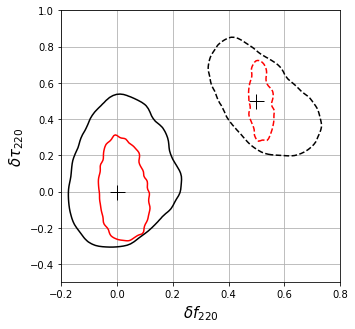
\includegraphics[width=0.3\textwidth]{figures/GW150914_GW190521_simulated_frac.png}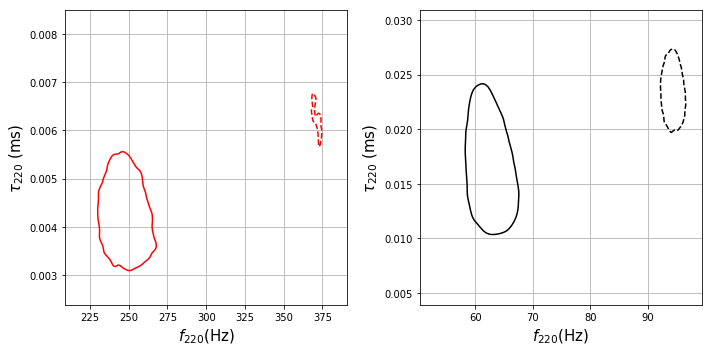
\includegraphics[width=0.56\textwidth]{figures/GW150914_GW190521_simulated_abs.png}\label{fig:gr_simulation}
	\caption{final figure will contain a third set of contours for modGR recovered assuming GR to show bias. That run is ongoing.}
\end{figure*}
%%%%%%%%%%%%%%%%%%%%%%%%%%%%%%%%%%%%%%%%%%%%%%%%%%%%%%%%%%%%%%%
%%%%%%%%%%%%%%%%%%%%%%%%%%%%%%%%%%%%%%%%%%%%%%%%%%%%%%%%%%%%%%%

\iffalse
\abhi{The GW150914-like injections we have:}
\begin{itemize}
\item{an SEOBNRv4HM software injection with the 22 mode frequencies estimated}
\item{a non-spinning NR injection with parameters close to the real event but higher SNR for which 22 mode frequencies are estimated}
\item{a non-spinning highly-asymmetric (q=6) NR injection with total mass similar to GW150914 and high SNR for which 22 and 33 mode frequencies are estimated}
\end{itemize}
\fi

\subsubsection{Test of the No hair theorem}

We provide a simple demonstration of a test of the no-hair theorem using our model. As described in the introduction, any test of the no-hair theorem of black holes would need to involve the independent measurements of (at least) two different QNMs. We use a simulated GW signal from the SXS catalog CITE corresponding a non-spinning binary black hole with a mass-ratio $q=6$ (SXS:BBH:0166), rescaled to a total mass of $M=84 \Mo$. We choose an asymmetric system to increase the SNR in the higher modes. We also rescale the distance and orientation of the binary such that the total SNR of the signal is 75. Based on the LIGO-Virgo observations during  O3, such asymmetric and loud signals are no longer just a theoretical prediction but quite the possibility at design sensitivities CITE of these detectors. Using the signal, we attempt to measure the QNM frequencies corresponding to the zeroeth overtone of the $(2,\pm 2)$ and $(3,\pm 3)$ modes~\ref{fig:nohair_sxs}. We explore two cases, where we fix either one of the $(2,\pm 2)$ or $(3,\pm 3)$ frequency and damping time, ie, $(f_{220}^{\text{eff}}, \tau _{220}^{\text{eff}})$ or $(f_{330}^{\text{eff}}, \tau _{330}^{\text{eff}})$ fixed at their GR predictions and estimating the other pair.

%%%%%%%%%%%%%%%%%%%%%%%%%%%%%%%%%%%%%%%%%%%%%%%%%%%%%%%%%%%%%%%
%%%%%%%%%%%%%%%%%%%%%%%%%%%%%%%%%%%%%%%%%%%%%%%%%%%%%%%%%%%%%%%
\begin{figure*}
	%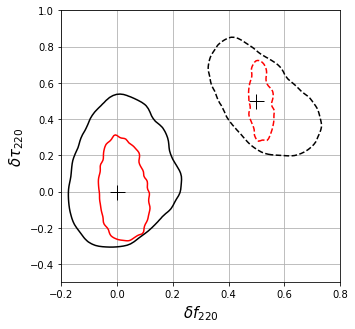
\includegraphics[width=0.3\textwidth]{figures/GW150914_GW190521_simulated_frac.png}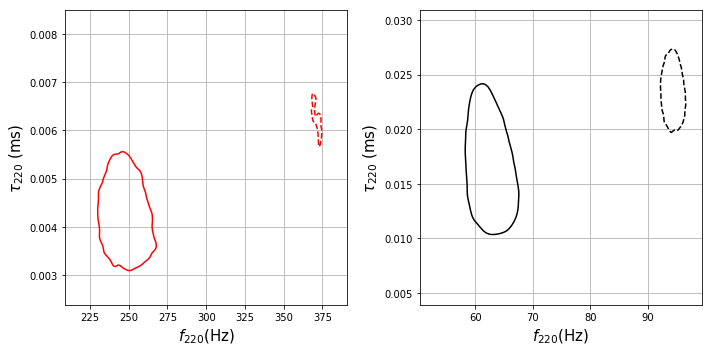
\includegraphics[width=0.56\textwidth]{figures/GW150914_GW190521_simulated_abs.png}
	\label{fig:nohair_sxs}
	\caption{SXS:BBH:0166. 220/330 measurement}
\end{figure*}
%%%%%%%%%%%%%%%%%%%%%%%%%%%%%%%%%%%%%%%%%%%%%%%%%%%%%%%%%%%%%%%
%%%%%%%%%%%%%%%%%%%%%%%%%%%%%%%%%%%%%%%%%%%%%%%%%%%%%%%%%%%%%%%

\iffalse
\abhi{As part of review we had developed the infrastructure to make non-GR waveforms using pSEOBNRv4HM, and running LALInference on it. We had specifically chosen an injection with domega220 = dtau220  = 0.5 in zero-noise, and successfully recovered those frequencies thus demonstrating the robustness of the method in detecting deviations from GR.}
\fi

\subsection{Simulations using nonGR signals}

To demonstrate the robustness of the method in detecting possible deviations of the underlying GW signal from predictions of GR, we inject simulated GW signals which are identical to the corresponding GR prediction upto merger \abhi{be more specific}, and differ in their post-merger description. We again choose systems with initial-binary-parameters similar to GW150914 and GW190521, but we attach a phenomenological post-merger signal described by deviation parameters $d\omega =d\tau = 0.5$. In other words, we assume that the frequency and damping time of our nonGR signal is 1.5 times the corresponding GR prediction, although the pre-merger signal is identical to GR (Fig.\ref{fig:nongr_waveform}). We also avoid waveform and noise systematic biases by choosing a configuration identical to the simulations described in Sec.\ref{ssec:gr_signal}. The posterior probability distributions on $\{d\omega,d\tau\}$ or equivalently $(f_{220}^{\text{eff}}, \tau _{220}^{\text{eff}})$ (dashed lines in Fig.\ref{fig:gr_simulation})) are consistent with the corresponding the values of the injection parameters, indicated by plus signs \abhi{add markers in effective quantity plots}.

%%%%%%%%%%%%%%%%%%%%%%%%%%%%%%%%%%%%%%%%%%%%%%%%%%%%%%%%%%%%%%%
%%%%%%%%%%%%%%%%%%%%%%%%%%%%%%%%%%%%%%%%%%%%%%%%%%%%%%%%%%%%%%%
\begin{figure}[H]
	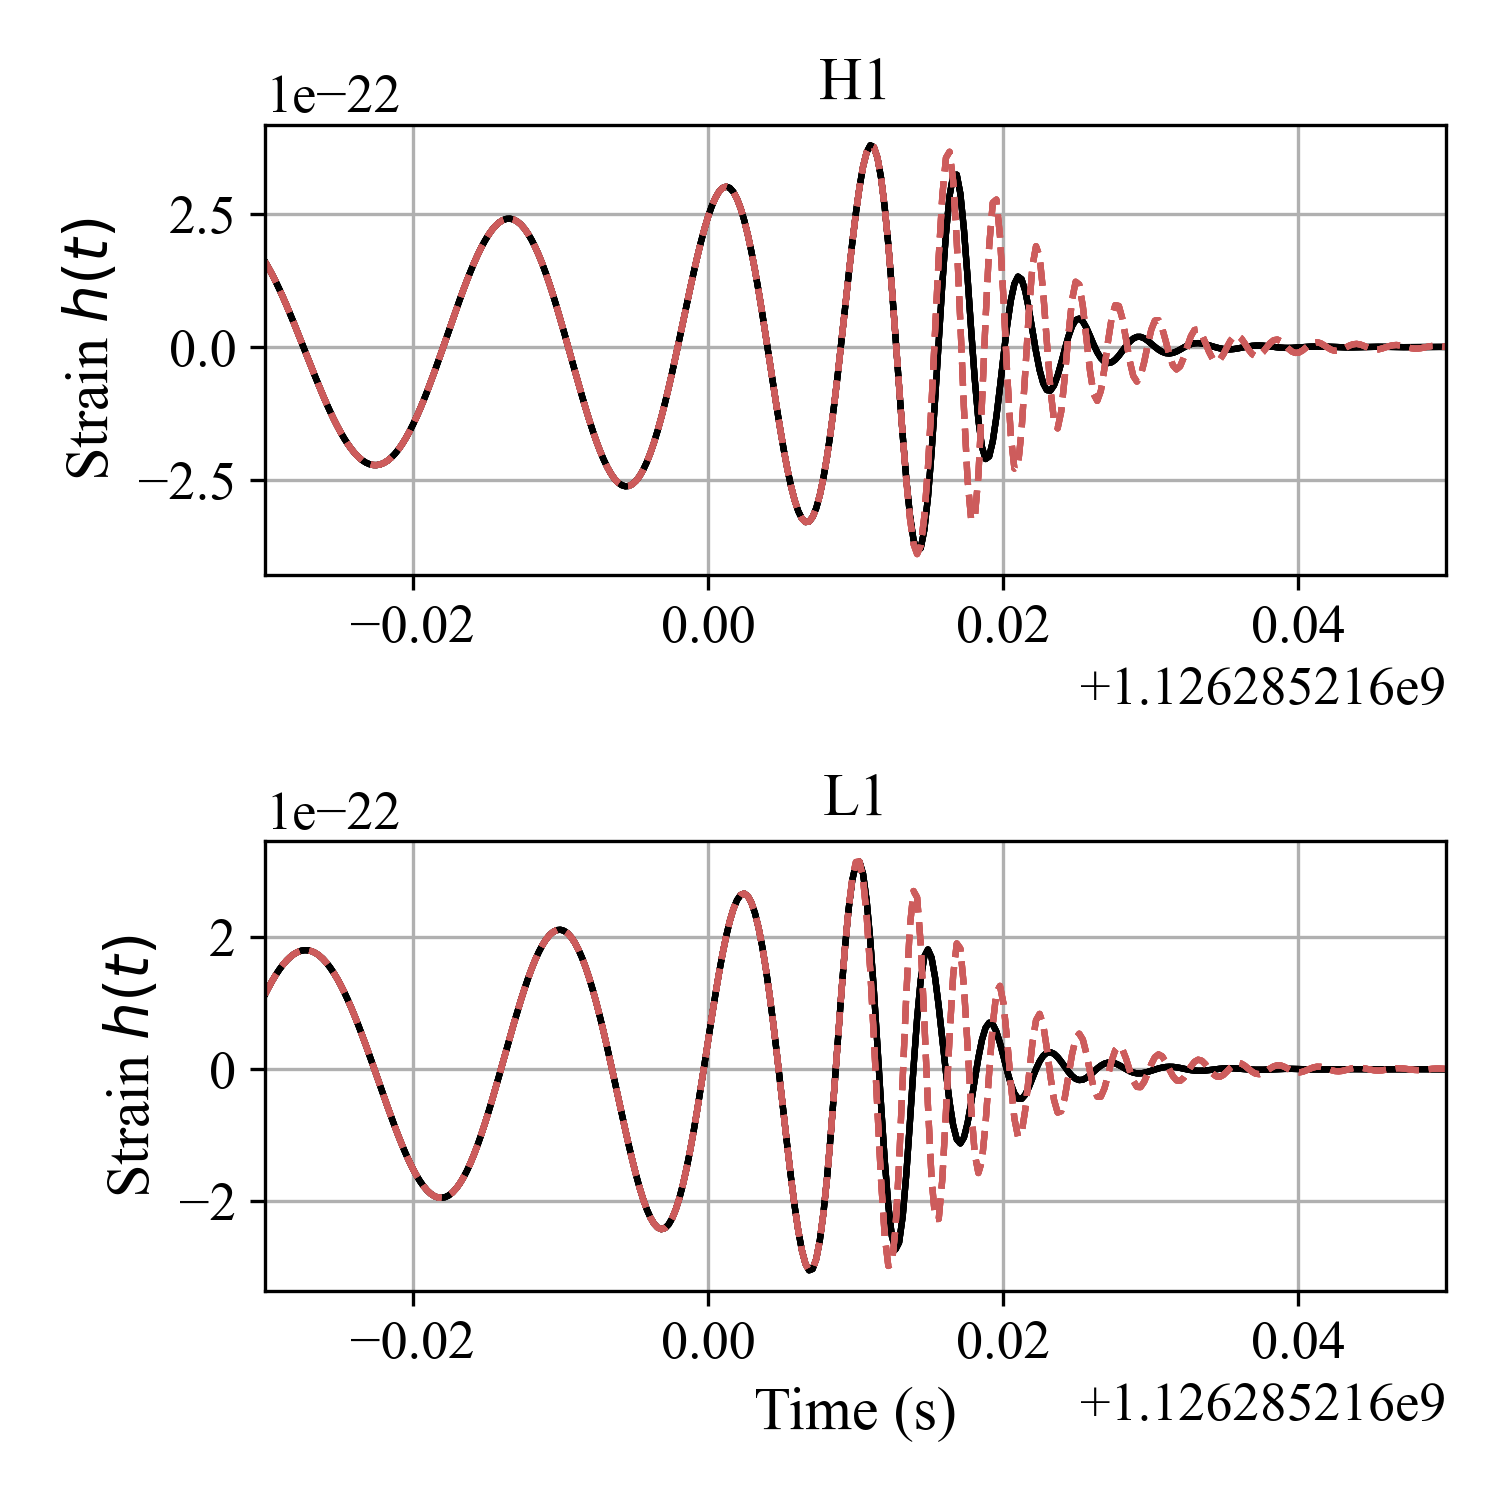
\includegraphics[width=0.5\textwidth]{figures/modGR_waveforms.png}\label{fig:nongr_waveform}
	\caption{NonGR waveforms}
\end{figure}
%%%%%%%%%%%%%%%%%%%%%%%%%%%%%%%%%%%%%%%%%%%%%%%%%%%%%%%%%%%%%%%
%%%%%%%%%%%%%%%%%%%%%%%%%%%%%%%%%%%%%%%%%%%%%%%%%%%%%%%%%%%%%%%

\subsection{Results on actual LIGO-Virgo results}

The LIGO-Virgo Collaboration recently released their testing GR catalog containing results of this test for all events observed during the first half of O3 CITE, which passed a threshold for the total detector frame mass > XX and SNRs in the pre- and post-merger regions to be atleast YY. For reasons of computational expense the analyses of the relevant events during the LIGO-Virgo's first and second observing runs could not be included in the catalog, and are being presented here for the first time. We conduct analysis on the 5 relevant events that pass the above thresholds from the O1-O2 catalog CITE: GW150914, GW170104, GW170729, GW170814 and GW170823 \abhi{what about GW170809?}. Out of these, the analysis of GW170814 and GW170823 return uninformative posteriors. This is because of an insufficient SNR In the post-merger signal for these two events. For GW170814, this is because the total mass is slightly lower than the rest, thus coalescing in the region of the detector bandwidth dominated by shot-noise, while in the case of GW170823 the overall SNR of the entire signal is too low to reliably estimate $\{d\omega,d\tau\}$. For the three remaining signals, GW150914, GW170104 and GW170729, we provide the posterior distributions in $\{d\omega,d\tau\}$ in the top panel of Fig.\ref{fig:o1o2_events}. We also reconstruct the effective QNM parameters, $(f_{220}^{\text{eff}}, \tau _{220}^{\text{eff}})$ which are tabulated in Table \ref{tab:qnm_o1o2_results}.

Among all GW signals detected so far, GW150914 is unique in it's loudness, mass as well as the clarity of the signal, leading to the first, and to date, best attempt in measuring the QNM frequencies CITE. The bottom panel of Fig.\ref{fig:o1o2_events} compares the results we obtain for GW150914 with previously published LIGO-Virgo results using a damped-sinusoid method, as well as the measurement reported using a non-spinning model in \paperone. The damped-sinusoid model assumed specific cutoff times (indicated in the curves on the bottom panel of Fig.\ref{fig:o1o2_events}) after the time corresponding to the peak amplitude as predicted by the best-fitting GR template waveform. Increasing time, decreasing SNR, wider posteriors, less-precise measurement. Compared to that we see when we incorporate the complete IMR version of the test, we utilise more SNR leading to tighter constraints.

%%%%%%%%%%%%%%%%%%%%%%%%%%%%%%%%%%%%%%%%%%%%%%%%%%%%%%%%%%%%%%%
%%%%%%%%%%%%%%%%%%%%%%%%%%%%%%%%%%%%%%%%%%%%%%%%%%%%%%%%%%%%%%%
\begin{figure}[H]
	\includegraphics[width=0.4\textwidth]{figures/O1O2_realevents.png}
	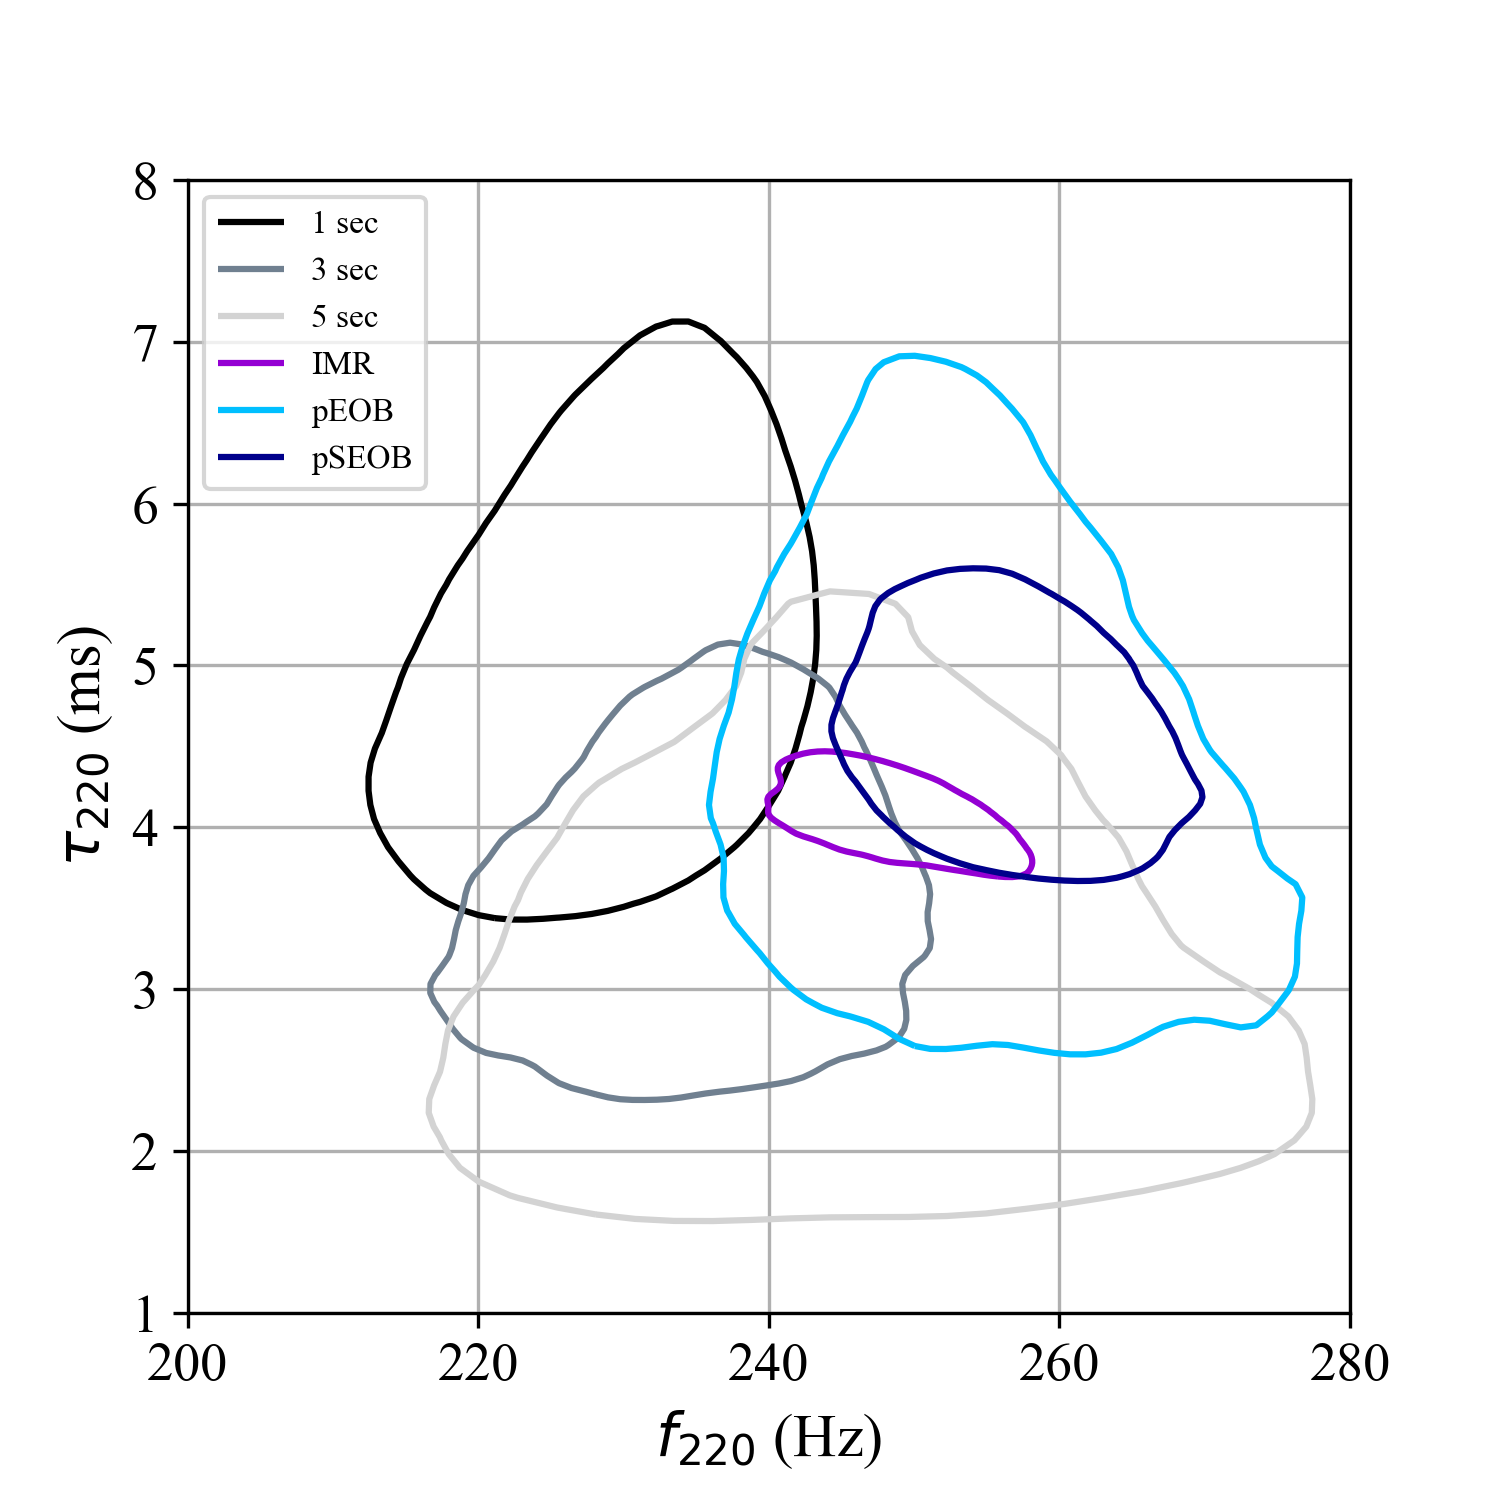
\includegraphics[width=0.4\textwidth]{figures/GW150914.png}
	\caption{O1-O2 analysis}\label{fig:o1o2_events}
\end{figure}
%%%%%%%%%%%%%%%%%%%%%%%%%%%%%%%%%%%%%%%%%%%%%%%%%%%%%%%%%%%%%%%
%%%%%%%%%%%%%%%%%%%%%%%%%%%%%%%%%%%%%%%%%%%%%%%%%%%%%%%%%%%%%%%

\begin{tabular}{llllllll}
\toprule
Event & \multicolumn{3}{c}{Redshifted} & \hphantom{X} & \multicolumn{3}{c}{Redshifted} \\
& \multicolumn{3}{c}{frequency [Hz]} & \hphantom{X} & \multicolumn{3}{c}{damping time [ms]} \\[0.075cm]
\cline{2-4}
\cline{6-8}
& IMR & DS & pSEOB & \hphantom{X} & IMR & DS & pSEOB \\
\midrule

GW150914 &
$249^{+9}_{-7}$ &
$247^{+14}_{-16}$ &
$-$ &
\hphantom{X} &
$4.1^{+0.3}_{-0.2}$ &
$4.8^{+3.7}_{-1.9}$ &
$-$
\\[0.075cm]

GW170104 &
$286^{+16}_{-27}$ &
$228^{+71}_{-102}$ &
$-$ &
\hphantom{X} &
$3.5^{+0.4}_{-0.3}$ &
$3.6^{+36.2}_{-2.1}$ &
$-$
\\[0.075cm]

GW170729 &
$161^{+13}_{-14}$ &
$148^{+11}_{-11}$ &
$-$ &
\hphantom{X} &
$7.8^{+1.8}_{-1.5}$ &
$10.4^{+8.2}_{-4.7}$ &
$-$
\\[0.075cm]

GW170814 &
$295^{+13}_{-12}$ &
$527^{+340}_{-332}$ &
$-$ &
\hphantom{X} &
$3.7^{+0.3}_{-0.2}$ &
$25.1^{+22.2}_{-19.0}$ &
$-$
\\[0.075cm]

GW170823 &
$199^{+14}_{-16}$ &
$222^{+664}_{-62}$ &
$-$ &
\hphantom{X} &
$5.4^{+1.0}_{-0.6}$ &
$13.4^{+31.8}_{-9.8}$ &
$-$
\\[0.075cm]

\bottomrule
\end{tabular}\label{tab:qnm_o1o2_results}

\subsection{Results on noise systematics study}

\iffalse
\abhi{A small summary of the noise systematics study that was done for S190521g to show that the deviations seen were consistent with systematics due to noise. The study include 2 separate sections: in Gaussian noise, and in real LIGO-Virgo noise immediately adjacent to the actual event.}
\fi

In order to investigate the 

%%%%%%%%%%%%%%%%%%%%%%%%%%%%%%%%%%%%%%%%%%%%%%%%%%%%%%%%%%%%%%%
%%%%%%%%%%%%%%%%%%%%%%%%%%%%%%%%%%%%%%%%%%%%%%%%%%%%%%%%%%%%%%%
\begin{figure}[H]
	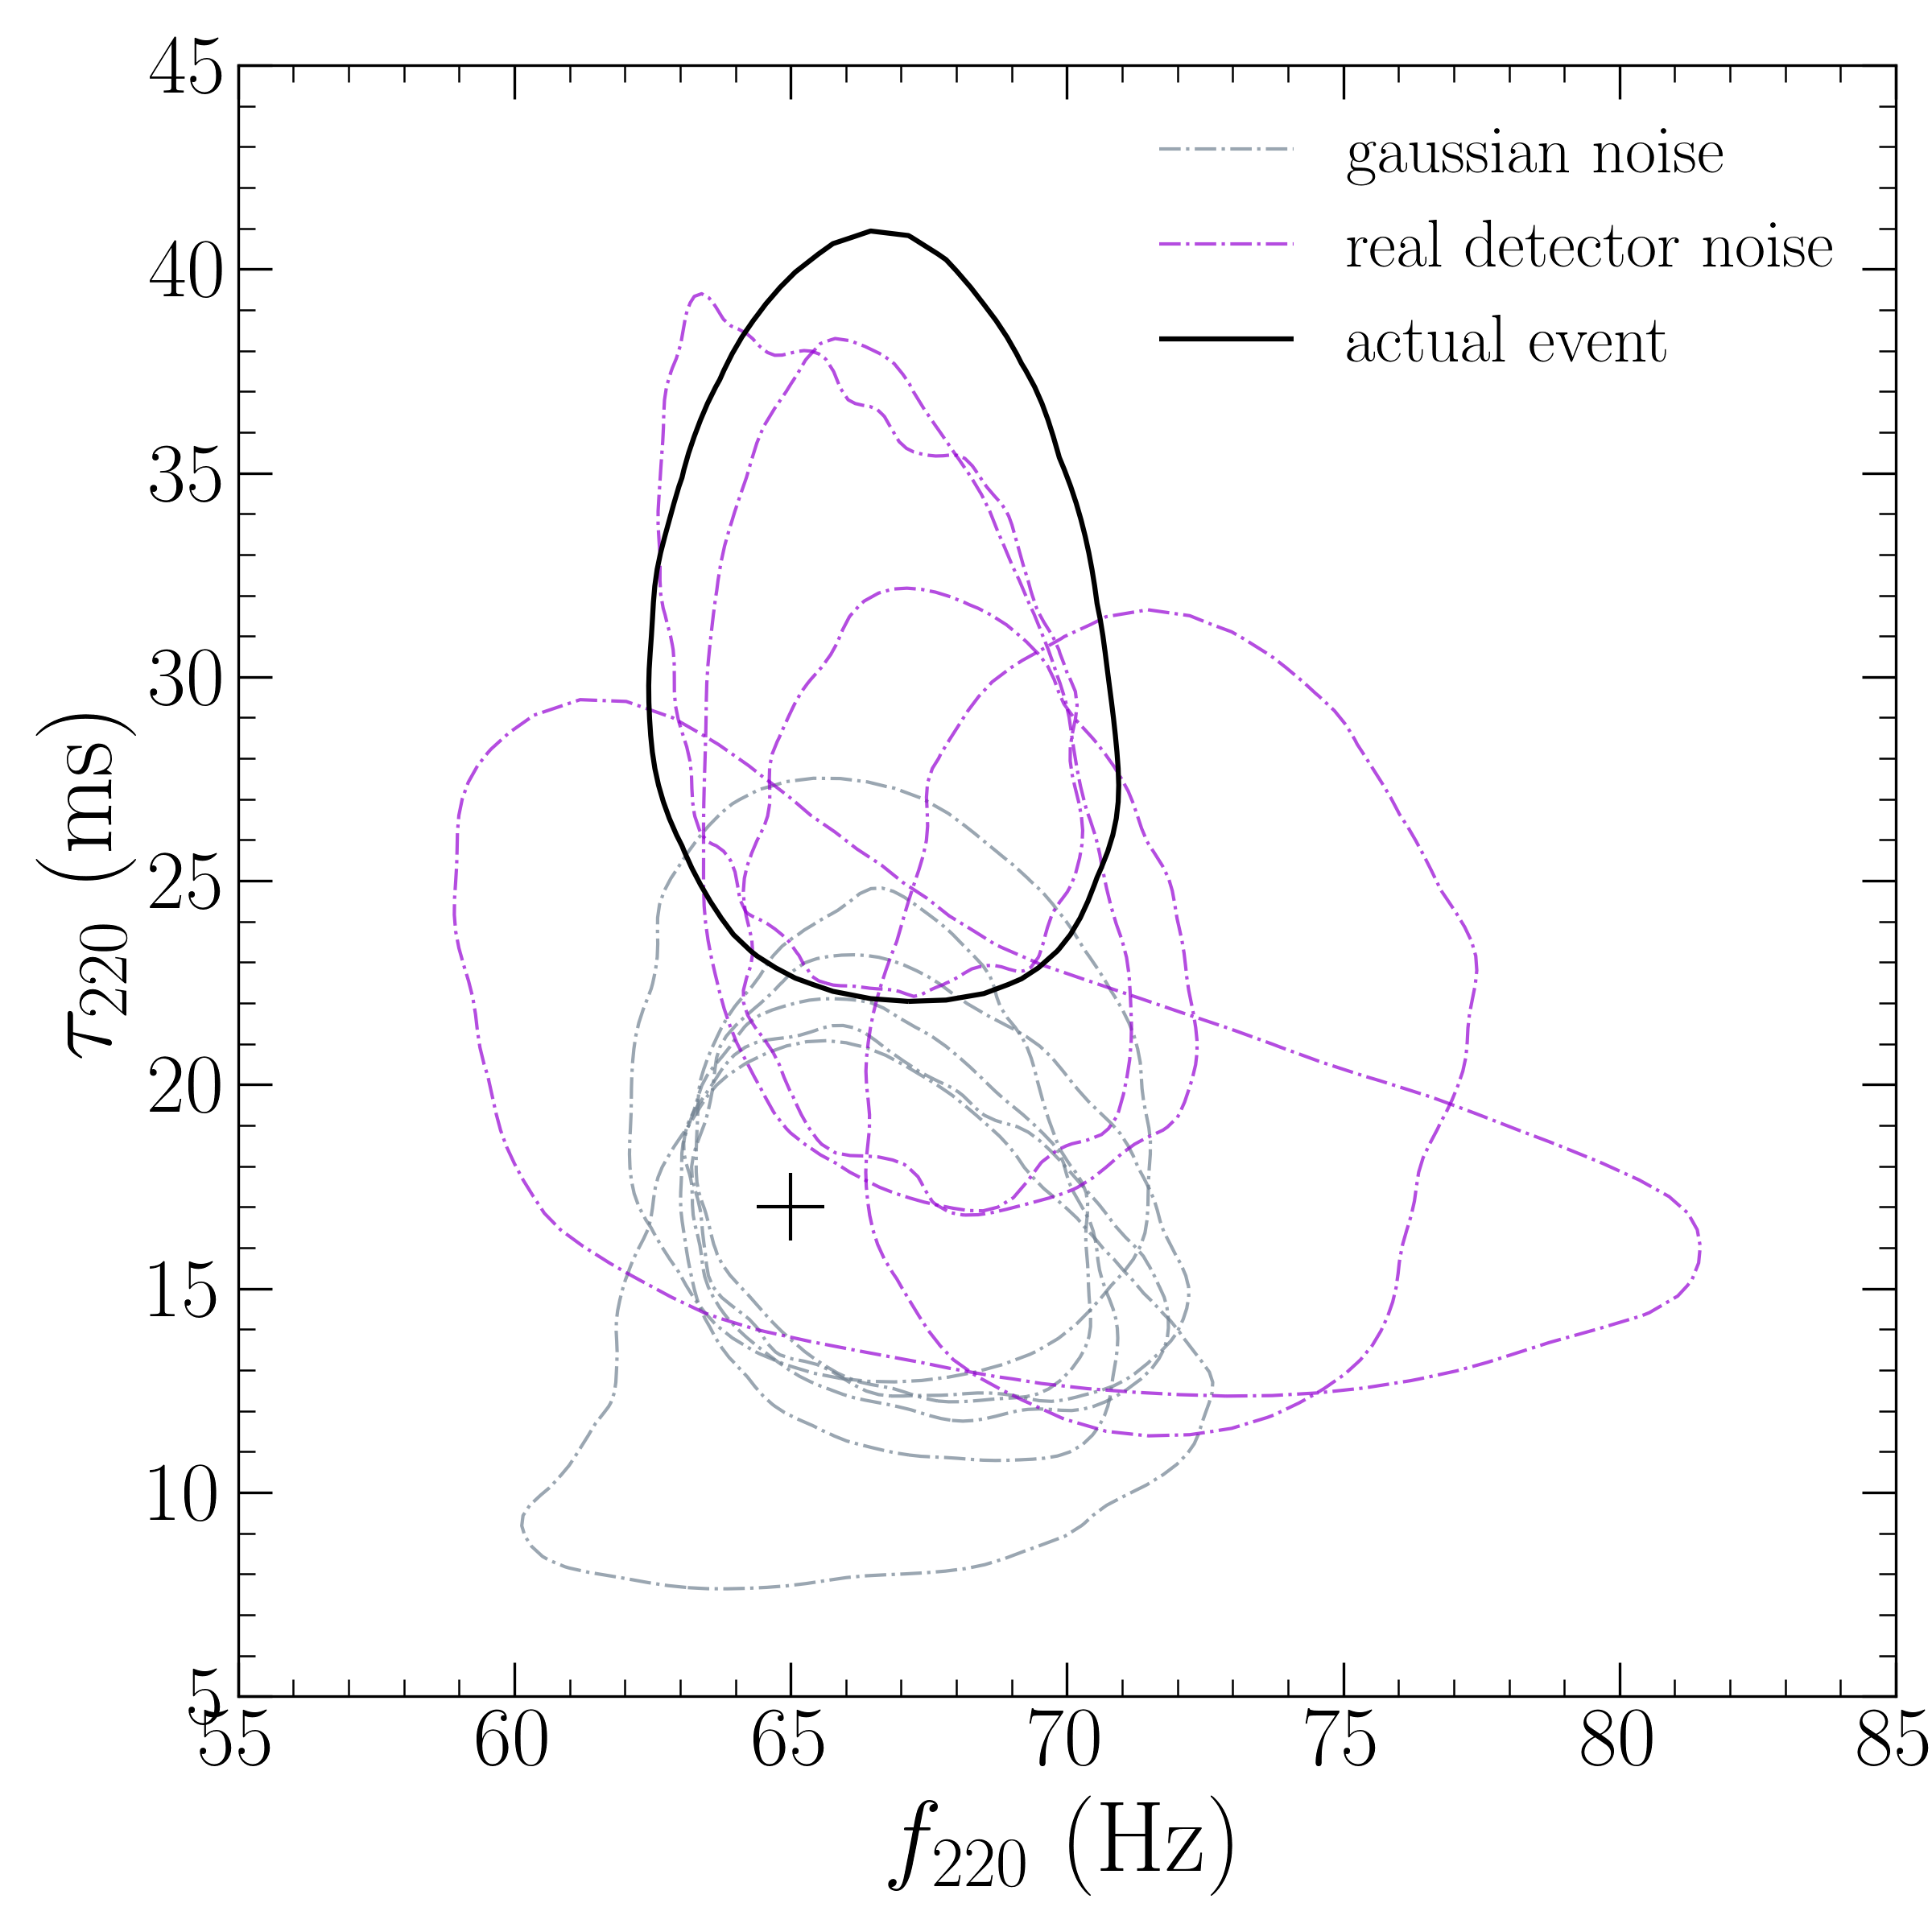
\includegraphics[width=0.4\textwidth]{figures/S190521g_swinjs.png}
	\caption{a single figure for both Gaussian and Real noise injections, color coded, to save space}\label{fig:21g_systematics}
\end{figure}
%%%%%%%%%%%%%%%%%%%%%%%%%%%%%%%%%%%%%%%%%%%%%%%%%%%%%%%%%%%%%%%
%%%%%%%%%%%%%%%%%%%%%%%%%%%%%%%%%%%%%%%%%%%%%%%%%%%%%%%%%%%%%%%

We injected NRSur7dq4 signal using the MaxL parameters from EXP30, in 2.5 hours of data surrounding the event at: t0-1.5 hours, t0-1., t0-0.5, t0+0.5, t0+1. For 3 of the 5 noise realisations, corresponding to t0-1 hour, t0+0.5 hours, and t0+1.0 hour we recover a damping time similar to the actual event, whereas for a third case, t0-0.5 hours, we obtain a damping time consistent at the 90\% credible interval (bottom panel of FIg.\ref{fig:21g_systematics}). L1-SNR goes down by more than 3 in some runs (maximum L1-SNR 12, minimum 9), indicative of how the noise variability is strongly affecting the recovered parameters. For some injections the mass ratio is biased, although final spin (most sensitive to mass ratio) is not affected much.  domega varies quite a lot among runs, instead dtau seems well behaved around zero. Effective frequency is a stable parameter (always well measured), while effective tau is much more sensitive to the noise configuration.  


\section{Discussion}\label{sec:discussion}

\iffalse
\abhi{A comparison with pyRING}
\abhi{damped sinusoid results}
\fi

%
\bibliographystyle{apsrev}
\bibliography{intro_paper}

\end{document}